\chapter{Evaluation}
\label{ch:evaluation}
To evaluate RDF-Doctor, firstly, it was tested against standard test cases, including formats of correct and incorrect syntax in files, secondly, to get rid of bias, a random number of errors was generated using Poisson distribution and uniform random number generators for a period of time of 8 hours to simulate a couple of syntax errors, produced by an ontology user, lastly, the performance of RDF-Doctor was measured when both the number of errors and the volumes of ontologies are varied. This chapter discusses all of such experiments in the following text. 
\section{Implementation}
Experiments were run on a Linux
Ubuntu 18.04 machine with a 4th Gen Intel Core i5-
4300U CPU, 3MB Cache, 2.90GHz with 8GB RAM
1333MHz DDR3. RDF-Doctor was implemented using
Java version 9. ANTLR framework version 4.7.1 was used to build the internal parser in RDF-Doctor, as well, as an imported library for compiling and running of it.  

\section{Experiment 1: Validating with RDF Suite Test} In this experiment, RDF-Doctor was validated against RDF Suite Test, specifically Turtle serialization. Next text discusses the objective, shows the implementation, and presents the result of the experiment.     
\subsection{Objective}
The evaluation phase starts with \citealp{TurtleTests:Online} where Test Suite files of Turtle serialization are found. There are multiple Test Suites for each of RDF serializations, recommend by W3 Consortium\footnote{https://www.w3.org/}. The proficiency of a parser for a certain serialization can be validated with these files found in a corresponding Test Suite . Files at \cite{TurtleTests:Online} were prompted to validate a parser that parses a Turtle serialization, hence, it was used to test RDF-Doctor. Metrics of the experiment are both Precision and Recall, donated by equation \ref{eq:1} and \ref{eq:1} sequentially. The former measures the percentage of errors which correctly flagged as syntax errors, while the latter calculates the percentage of actual syntax errors which correctly recognized. 

\subsection{Result and Discussion}

The test drives the result when dealing with either correct or incorrect Turtle syntax. Thus, correct syntaxes should be recognized as correct, similarly in case of incorrect syntaxes plus exception errors should be fired.  However,  the test result in Table \ref{tab:TurtleSuit} shows recognizes mostly of correct syntaxes with 88\%, while the remaining 12\% RDF-Doctor are not recognized and it consider them as errors. In the meanwhile, when dealing with incorrect syntaxes, again, Table \ref{tab:TurtleSuit} provides that 81,5\% of files included incorrect syntaxes are detected and an error message was fired for each one of them, the rest 17,5\% go without being identified as incorrect forms, as well as no errors were fired.



\begin{table}[]
\centering
\begin{tabular}{|l|l|l|l|}
\hline
\begin{tabular}[c]{@{}l@{}}Error Type Classification \end{tabular} & Detected & \begin{tabular}[c]{@{}l@{}}Not detected\end{tabular} & Total \\ \hline
 Escape Characters              &      0    &    4 &   4  \\ \hline
 Bad Keywords             &      5   &    0 &   5  \\ \hline
 Bad Literals with langTag             &      2   &    0 &   2  \\ \hline
 Bad Local Name-space in IRI             &      2   &    3  &   5  \\ \hline
 Bad Namespace in IRI             &      2   &    0 &   2  \\ \hline
 N3 Extra             &      11   &    1 &   12  \\ \hline
 Bad Namespace in Directives             &      2   &    0 &   2  \\ \hline
 Bad Number as a Literal             &      5   &    0 &   5  \\ \hline
 Bad Directives             &      4   &    0 &   4  \\ \hline
 Bad Strings             &      6   &    1 &   7  \\ \hline
 Bad Structures            &      12   &    0 &   12  \\ \hline
 Bad IRI            &      2   &    3 &   5  \\ \hline
 Total            &      53   &    12 &   65  \\ \hline
\end{tabular}
\caption{\textbf{Evaluation of RDF-Doctor against detection of incorrect syntaxes in Turtle Test Suite \cite{TurtleTests:Online}.} The test focused on the files, included with an incorrect Turtle syntax.}
\label{tab:detection}
\end{table}
\begin{table}[]
\centering
\begin{tabular}{|l|l|l|l|l|}
\hline
\begin{tabular}[c]{@{}l@{}}File Content \end{tabular} & Detected & \begin{tabular}[c]{@{}l@{}}Not detected \\ without errors \end{tabular} &\begin{tabular}[c]{@{}l@{}} Not detected \\ with errors \end{tabular}  & Total \\ \hline
 Correct Syntax              &      185    &    0 &   25  & 210 \\ \hline
 Incorrect/Bad Syntax              &      53    &    12 &   0  & 65 \\ \hline
 Total            &      238   &    12 &   25 & 275  \\ \hline
\end{tabular}
\caption{\textbf{ Evaluation summary of RDF-Doctor for both correct and incorrect syntaxes when validating with Turtle Test Suite \cite{TurtleTests:Online}.} }
\label{tab:TurtleSuit}
\end{table}
For evaluation, the precision and recall are computed using the equations \ref{eq:1} and \ref{eq:2} respectively.  
\begin{align} 
   Precision=  \frac{t_p}{t_p+f_p}\,;\qquad
\qquad\parbox{4.0cm}{\footnotesize$\begin{aligned} t_p &= \text{ number of true positives}\\[-1.0ex] f_p &= \text{ number of false positives}\end{aligned}$}
   \label{eq:1}
\end{align}

   
\begin{align}
   Recall =  \frac{t_p}{t_p+f_n} \,;\qquad
\qquad\parbox{4.0cm}{\footnotesize$\begin{aligned} t_p &= \text{ number of true positives}\\[-1.0ex] f_n &= \text{ number of true negatives}\end{aligned}$}
   \label{eq:2}
\end{align}

\begin{figure}[ht]
\begin{center}
		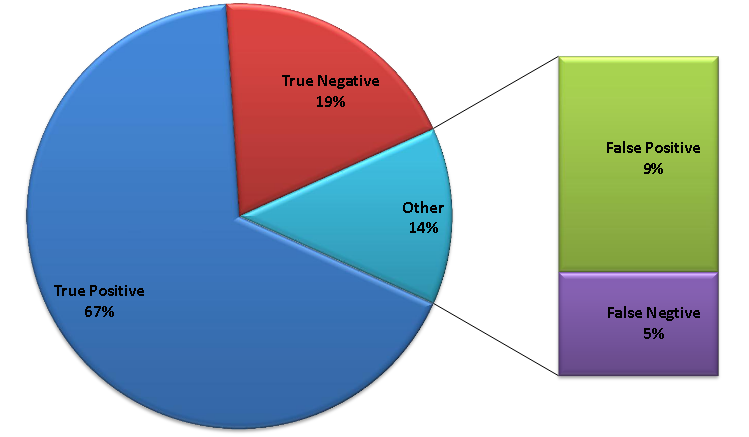
\includegraphics[scale=0.5,angle=0]{images/PieChartExperiment1.png}

		\label{Fig:pieChartExperiment1}
		\caption{\textbf{Result of Experiment 1 to evaluate  RDF-Doctor using Turtle Test Suite \cite{TurtleTests:Online}.}}
\end{center}
\end{figure}

\section{Experiment 2: Random Syntax Errors Generation}
\subsection{Objective}




\subsection{Result and Discussion}

In this experiment, number of syntax errors are arbitrarily created using a Poisson Distribution, for example. a user who is working on on RDF data for 8 hours and each one hour he is making a change (insert/modify/delete a text) is simulated. The average number of making syntax errors per time interval is represented by the parameter $\lambda$ . To make more clear, if   $\lambda$ = 5, it means that five syntax errors were occurred per hour.  Assuming a user can introduce 10 syntax error per hour

	\begin{figure}[ht]
	\begin{center}
		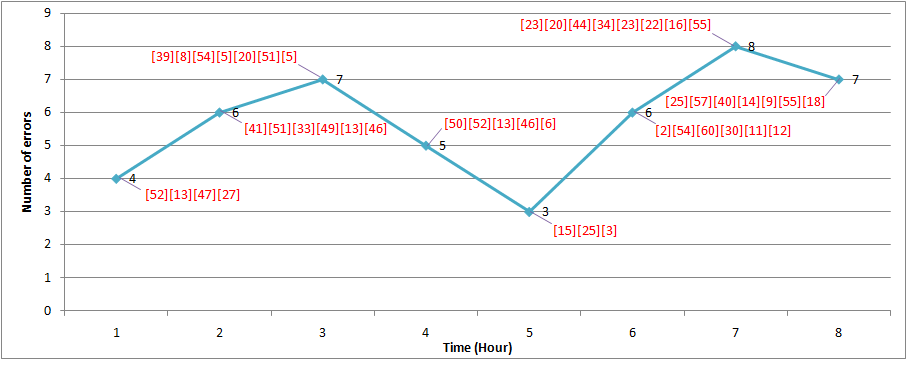
\includegraphics[scale=0.58,angle=0]{images/experiment2.png}
				\setlength\belowcaptionskip{-5mm}
		\caption{\textbf{Random Syntax Errors Distribution.} Number and types of syntax errors between brackets for a user in an interval of 8 hours. A Poisson  distribution with $\lambda$ = 5 models an average of 5 syntax errors per hour. A uniform distribution is computed to represent the type of errors.} 
		\label{Fig:experiment2}
	\end{center}
\end{figure}



	\begin{figure}[ht]
	\begin{center}
		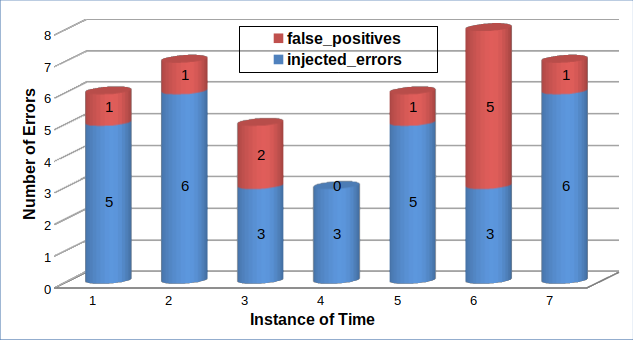
\includegraphics[scale=0.8,angle=0]{images/Experiment02-02.png}
				\setlength\belowcaptionskip{-5mm}
		\caption{\textbf{Result of error detection when syntax errors are randomly generated.}} 
		\label{Fig:Experiment02-02}
	\end{center}
\end{figure}

	\begin{figure}[ht]
	\begin{center}
		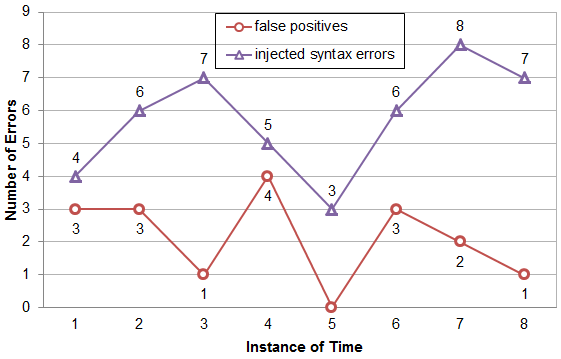
\includegraphics[scale=0.8,angle=0]{images/Experiment02-03.png}
				\setlength\belowcaptionskip{-5mm}
		\caption{\textbf{Result of False Positives when syntax errors are randomly generated.}} 
		\label{Fig:Experiment02-03}
	\end{center}
\end{figure}

\section{Experiment 3: Impact of Numbers of Errors and RDF Volume on Performance}
\subsection{Objective}

To evaluate the performance of the proposed solution, this experiment will be held where number of syntax errors and RDF input data are varied. Two types of anthologies are used: small and medium size ones.  




\subsection{Result and Discussion}







